\section{Modeling Path Planning as a MILP problem}
This section covers how a trajectory planning problem can be represented as a MILP problem. The problem representation is based on the work by Bellingham\cite{Bellingham2002}.
% \subsection{Overview of MILP}
% \label{subsec:previous}
MILP is an extension of linear programming. In a linear program, decision variables are unknown real numbers and the goal is to maximize or minimize a linear objective function subjected to a number of linear equality or inequality constraints. In MILP, some or all decision variables can be integers, which allows more flexibility in modeling at computational cost.

% There is a single (linear) objective function which needs to be minimized or maximized. A problem typically also contains a number linear inequalities which constrain the values of the variables in the objective function. When some (or all) of the variables are integers, the problem is a mixed integer problem. \\
% More complex mathematical relations can be modeled by combining multiple constraints. Some of those relations, like logical operators or the absolute value function, can only be expressed when integer variables are allowed \cite{Mitra1994}.
\subsection{Time and UAV state}
\label{section:modeling}
\begin{figure}
    \centering
        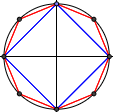
\includegraphics[width=0.33\columnwidth]{img/circlelinear2}
    \caption{If the velocity is limited to a finite value, the velocity vector must lie within the circle centered on the origin with the radius equal to that value. This is represented by the black circle. The blue and red polygons show the linear approximation using 4 and 8 constraints respectively.}\label{fig:circlelinear}
\end{figure}
The trajectory planning problem can be represented with $N$ discrete time steps and a set of state variables at each time step \cite{Bellingham2002}. The number of time steps determines the maximum amount of time the UAV has to reach its goal. 
% The actual movement of the UAV is modeled by the acceleration, velocity and position at each time step.
% based on the state variables from the previous time step. 
% There are $N + 1$ time steps, with a fixed amount of time $\Delta t$ between them.
\begin{equation}
\label{eq:p-start}
\boldsymbol{p}_0 = \boldsymbol{p}_{start}
\end{equation}
\begin{equation}
\label{eq:p-rest}
\boldsymbol{p}_{n+1} = \boldsymbol{p}_{n} + \Delta t * \boldsymbol{v}_{n}  \quad 0 \leq n < N - 1
\end{equation}
Eq. (\ref{eq:p-start}) and (\ref{eq:p-rest}) represent the state of the UAV at each time step. For each time step $n$, the position in the next time step $p_{n+1}$ is determined by the current position $p_n$, the current velocity $v_n$ and the time step size $\Delta t$. Velocity, acceleration and other derivatives are represented the same way. The number of derivatives needed depends on the specific use case.
\subsection{Objective function}
The objective is to minimize the time before the UAV reaches the goal position.
\begin{equation}
\label{eq:goal-fun}
\text{minimize} \quad - \mathlarger{\sum}_{n=0}^{n \leq N - 1} done_n
\end{equation}
Eq. (\ref{eq:goal-fun}) shows the objective function \cite{Bellingham2002}. Reaching the goal causes a state transition from not being done to being done. This is represented as the value of binary variable $done_n$. When $done_n = 1$, the UAV has reached its goal on or before time step $n$.
\begin{equation}
\label{eq:fin-start}
done_0 = 0, \quad done_{N - 1} = 1
\end{equation}
\begin{equation}
\label{eq:fin-rest}
done_{n+1} = done_n \vee cdone_{n+1},  \quad 0 \leq n < N - 1
\end{equation}
Eq. (\ref{eq:fin-start}) states that the UAV must reach its goal eventually. 
Lamport's state transition axiom method \cite{Lamport1989} was used to model state transitions. In Eq. (\ref{eq:fin-rest}), the state will be done at time step $n+1$ if the state is done at time step $n$ or if there is a state transition from not done to done at time step $n + 1$, represented by $cdone_{n+1}$.
%\begin{equation}
%\label{eq:cfin}
%cdone_n =  cdone_{p,t} \wedge \neg done_n\quad 0 \leq n \leq N
%\end{equation}
% $cdone_n$ in (\ref{eq:cfin}) is true at time step $n$ if the goal position requirement $cdone_{p,n}$ is true and the done state has not already been reached ( $ \neg done_n$ ). Additional constraints on the state transition, like a maximum velocity, can be added here.
\begin{equation}
\label{eq:cfin-p}
cdone_n = |x_{n} - x_{goal}| < \epsilon_{p} \wedge  |y_{n} - y_{goal}| < \epsilon_{p}, 0 \leq n < N
%cdone_{n} =  \mathlarger{\mathlarger{\bigwedge_{i = 0}^{i < Dim(\boldsymbol{p}_n)}}} |p_{n,i} - p_{goal, i}| < \epsilon_{p},  \quad 0 \leq n \leq N
\end{equation}
The goal position requirement is fulfilled if the UAV is closer than $\epsilon_p$ to the goal position in both dimensions \cite{Bellingham2002}.
%The goal position requirement is represented by $cdone_{p,n}$ and is satisfied when $cdone_{p,n} = 1$. The coordinate in dimension $i$ of the position vector $\boldsymbol{p}_n$, is $p_{n,i}$. The goal position coordinate in that dimension is $p_{goal, i}$. If the difference between those values is smaller than some value $\epsilon_p$ in every dimension at time step $n$,  $cdone_{p,n} = 1$.
\subsection{UAV state limits}
Modeling the maximum velocity of a UAV requires calculating the the velocity vector's 2-norm which is non-linear. However, the maximum velocity constraint can be approximated to an arbitrary degree using multiple linear constraints \cite{Bellingham2002}. Fig. \ref{fig:circlelinear} shows a visual representation of this approximation. The acceleration and other vector properties of the UAV can be limited in the same way.
%With $x_i$ and $y_i$ the $N_{points}$ vertices of the approximating polygon listed in counter-clockwise order, the velocity can be limited to $v_{max}$ with Eq. (\ref{eq:vmax}). 
%\label{eq:vmax}
%v_{n, 1} \leq a_i v_{n,0} + b_i  \quad 0 \leq i < N_{points}, ~ 0 \leq n \leq N
%\end{equation}

\subsection{Obstacle avoidance}
\begin{figure}[!t]
    \centering
    
    \begin{subfigure}[t]{0.35\columnwidth}
        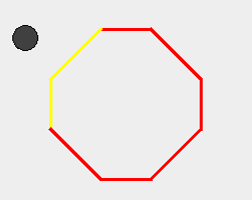
\includegraphics[width=\textwidth]{img/obs1c}
        \caption{}
        \label{fig:obs-clear}
    \end{subfigure}
    \begin{subfigure}[t]{0.35\columnwidth}
        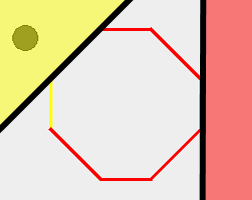
\includegraphics[width=\textwidth]{img/obs2c}
        \caption{}
        \label{fig:obs-regions}
    \end{subfigure}
    \caption{A visual representation of how obstacle avoidance works. Fig. \ref{fig:obs-clear} shows the UAV's current position as the black circle. The color of the edges of the obstacle represent whether or not the UAV is in the safe zone for that edge. An edge is yellow if the UAV is in the safe zone, and red otherwise. Fig. \ref{fig:obs-regions} shows the safe zones defined by a yellow and red edge in yellow and red respectively. }\label{fig:obs}
\end{figure}
The most challenging part of the problem is modeling obstacles. Any obstacle between the UAV and its goal will inherently make the search space non-convex. Because of this, integer variables are needed to model obstacles. 
Assuming that obstacles are convex polygons, for each obstacle, the UAV needs to be on the ``safe'' side of at least one edge to not collide with the obstacle (see Fig. \ref{fig:obs}). 
% For each edge of a polygon obstacle, the line through that edge is constructed. If the obstacle is convex, the obstacle will be entirely on one side of that line. This means that the other side can be considered a safe area. 
% However, the UAV cannot be in the safe area of all edges at the same time, so a mechanism is needed to turn off these constraints when needed. 
% To not collide with the obstacle, the UAV needs to be in the safe area of at least one edge (see Fig. \ref{fig:obs}). \\
Indicator constraints were used to model obstacle avoidance. This requires one boolean variable $slack$ per edge. If $slack$ is false, the UAV is on the safe side of the edge. For each obstacle at least one of the $slack$ variables need to be false. For every convex obstacle $o$ with the coordinates of vertex $i$ being $x_{o,i}$ and $y_{o,i}$ \cite{Bellingham2002}:
\begin{equation*}
dx_{o,i} = x_{o,i} - x_{o,i-1}, \quad dy_{o,i} = y_{o,i} - y_{o,i-1} 
\end{equation*}
\begin{equation*}
\label{eq:lin-a}
a_{o,i} = \dfrac{dy_{o,i}}{dx_{o,i}}, \quad b_{o,i} = y_{o,i} - a_{o,i} x_{o,i} \quad 0 \leq i < N_{vertices}
\end{equation*}
\begin{equation}
\label{eq:obs}
slack_{o,i,n} \Rightarrow \\
\begin{cases}
b_{o,i} \leq p_{n,y} - a_{o,i} p_{n,x} & dx_{o,i} < 0 \\
b_{o,i} \geq p_{n,y} - a_{o,i} p_{n,x} & dx_{o,i} > 0 \\
\end{cases}
\end{equation}
\begin{equation}
\neg \mathlarger{\mathlarger{\bigwedge_{i}}} slack_{o,i,n} \quad 0 \leq n < N
\end{equation}
Modeling obstacles this way is problematic because an integer variable is needed for every edge of every obstacle, for every time step. Each integer variable makes the solution space less convex, increasing the worst case execution time exponentially \cite{DBLP:conf/coco/Karp72}.